\documentclass[11pt]{beamer}

\usepackage[utf8]{inputenc}
\usepackage[english]{babel}
\usepackage{amsmath}
\usepackage{amsfonts}
\usepackage{amssymb}
\usepackage{graphicx}
\usetheme{Berkeley}
\newcommand\etal{\mbox{\textit{et al.}}}
\colorlet{mystruct}{structure} % Save current structure
\colorlet{structure}{brown} % New structure
\usestructuretemplate{\color{structure}}{} % \structure{..}
\beamertemplateshadingbackground{green!25}{blue!25} % New background

\author{Ruben \textsc{Espeleta Bolivar}\\ \and {Advisor: Dr. Cruz \textsc{García Molina}}}
\title{Numerical experiments of glacial inceptions in Northern Europe}
%\subtitle{}
%\logo{}
\institute{Institut des geosciences de l'environnement}
\date{\small{January 30th 2023}}
\titlegraphic{
\includegraphics[height=1cm]{../fig/logo_IGE.png}\hspace{0,3cm}
\includegraphics[height=1cm]{../fig/logo_UGA.png}\hspace{0,3cm} }
%\subject{}
%\setbeamercovered{transparent}
%\setbeamertemplate{navigation symbols}{}
\usecolortheme{orchid}

\begin{document}
 \begin{frame}
	\titlepage
\end{frame}
%%%%%%%%%%%%%%%%%%%%%%%%%%%%%%%%%%%%%%%
\section{Northern Europe}
%%%%%%%%%%%%%%%%%%%%%%%%%%%%%%%%%%%%%%%
\frametitle{Northern Europe}
	\begin{frame}
		\frametitle{Northern Europe}
		\begin{center}
			 \begin{figure}[!h]
				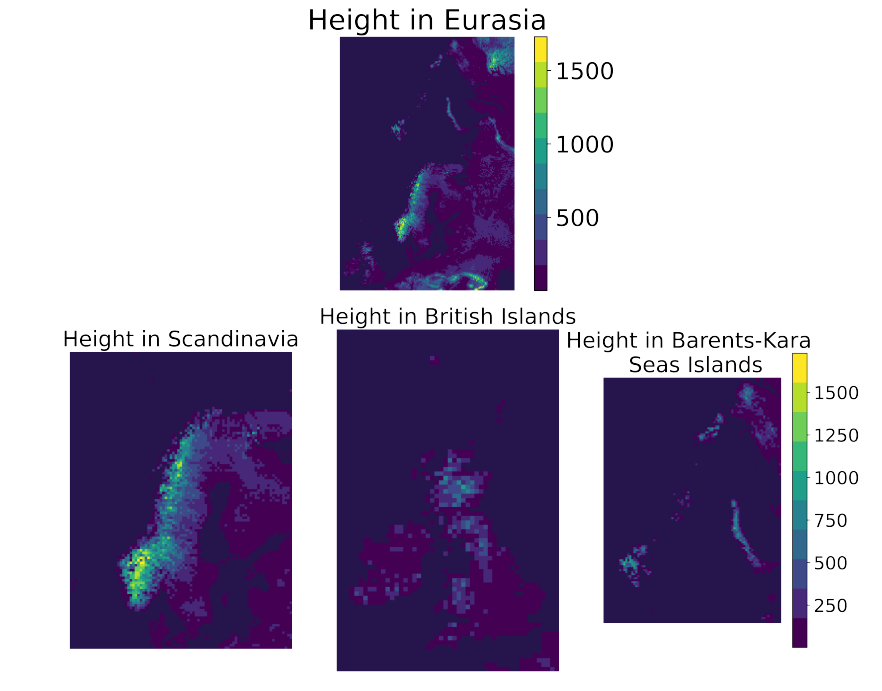
\includegraphics[width=0.6\textwidth]{../fig/Northern_europe.png} % \\\includegraphics[width=0.5\textwidth]{topography_x-profile.png}\includegraphics[width=0.5\textwidth]{topography_y-profile.png}
				\caption{\footnotesize Elevation of the terrain in Eurasia in meters. The top row shows the topography used by Dainche (2022) for his study. On the second row, zooms have been performed on regions where glacial inceptions started. Plotted from the data from ETOPO1 projected into a cartesian grid at 20km resolution. }
			\end{figure}
		\end{center}
	\end{frame}
\begin{frame}
	\frametitle{Idealised Northern Europe topography by Dainche (2022)}
			\begin{center}
		\begin{figure}[!h]
			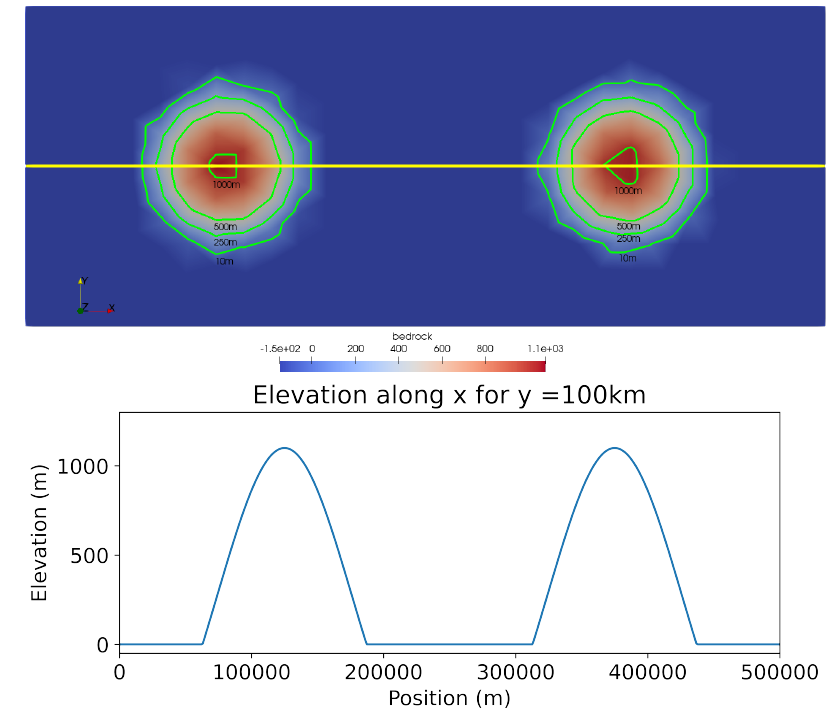
\includegraphics[width=0.7\textwidth]{../fig/Erwan_topography.png} % \\\includegraphics[width=0.5\textwidth]{topography_x-profile.png}\includegraphics[width=0.5\textwidth]{topography_y-profile.png}
			\caption{\footnotesize Topography of idealised system made of two Gaussian shaped mountains carried out by Dainche (2020). }
		\end{figure}
	\end{center}
\end{frame}
\begin{frame}
	\frametitle{Glaciers dynamics}
	For large time scales the ice is considered as a very viscous fluid. The ice flow equations are then derived from the Stokes equation:
	\begin{equation}
		div\sigma + \rho g = div\tau - gradp + \rho g = 0;
	\end{equation}
	with $\sigma$ the stress tensor, $\rho$ the density of the ice, g the gravity vector, $\tau$ the deviatoric stress tensor, with $\sigma = \tau - pI$ and $p=\frac{tr\sigma}{3}$. 
	And the mass conservation:
	\begin{equation}
		\frac{dh}{dt}+ div(uH)=M_s + M_b;
	\end{equation}
	With $u$ the velocity, H the ice thickness, $M_s$ and $M_b$ the mass balance at the surface and at the bottom respectively. $M_s$ will be defined, and $M_b$ is considered as 0 for convenience purposes. 
\end{frame}
\begin{frame}
	\frametitle{Glaciers dynamics}
	The stresses are related to the viscosity and the strain by the Glen's law:
	\begin{equation}
		\tau = 2\eta\dot{\epsilon},
	\end{equation}
	with the viscosity given by:
	\begin{equation}
		\eta = \frac{1}{2}(EA)^\frac{-1}{n} \dot{\epsilon_e}^\frac{(1-n)}{n}.
	\end{equation}
	Where:
	\begin{itemize}
		\item The strain rate $\dot{\epsilon}$.
		\item Glen's constant.
		\item The enhancement factor to account for an anisotropic effect E.
		\item The rheological parameter A.
	\end{itemize}
\end{frame}
\begin{frame}
	\frametitle{Grounding line}
		\begin{center}
		\begin{figure}[!h]
			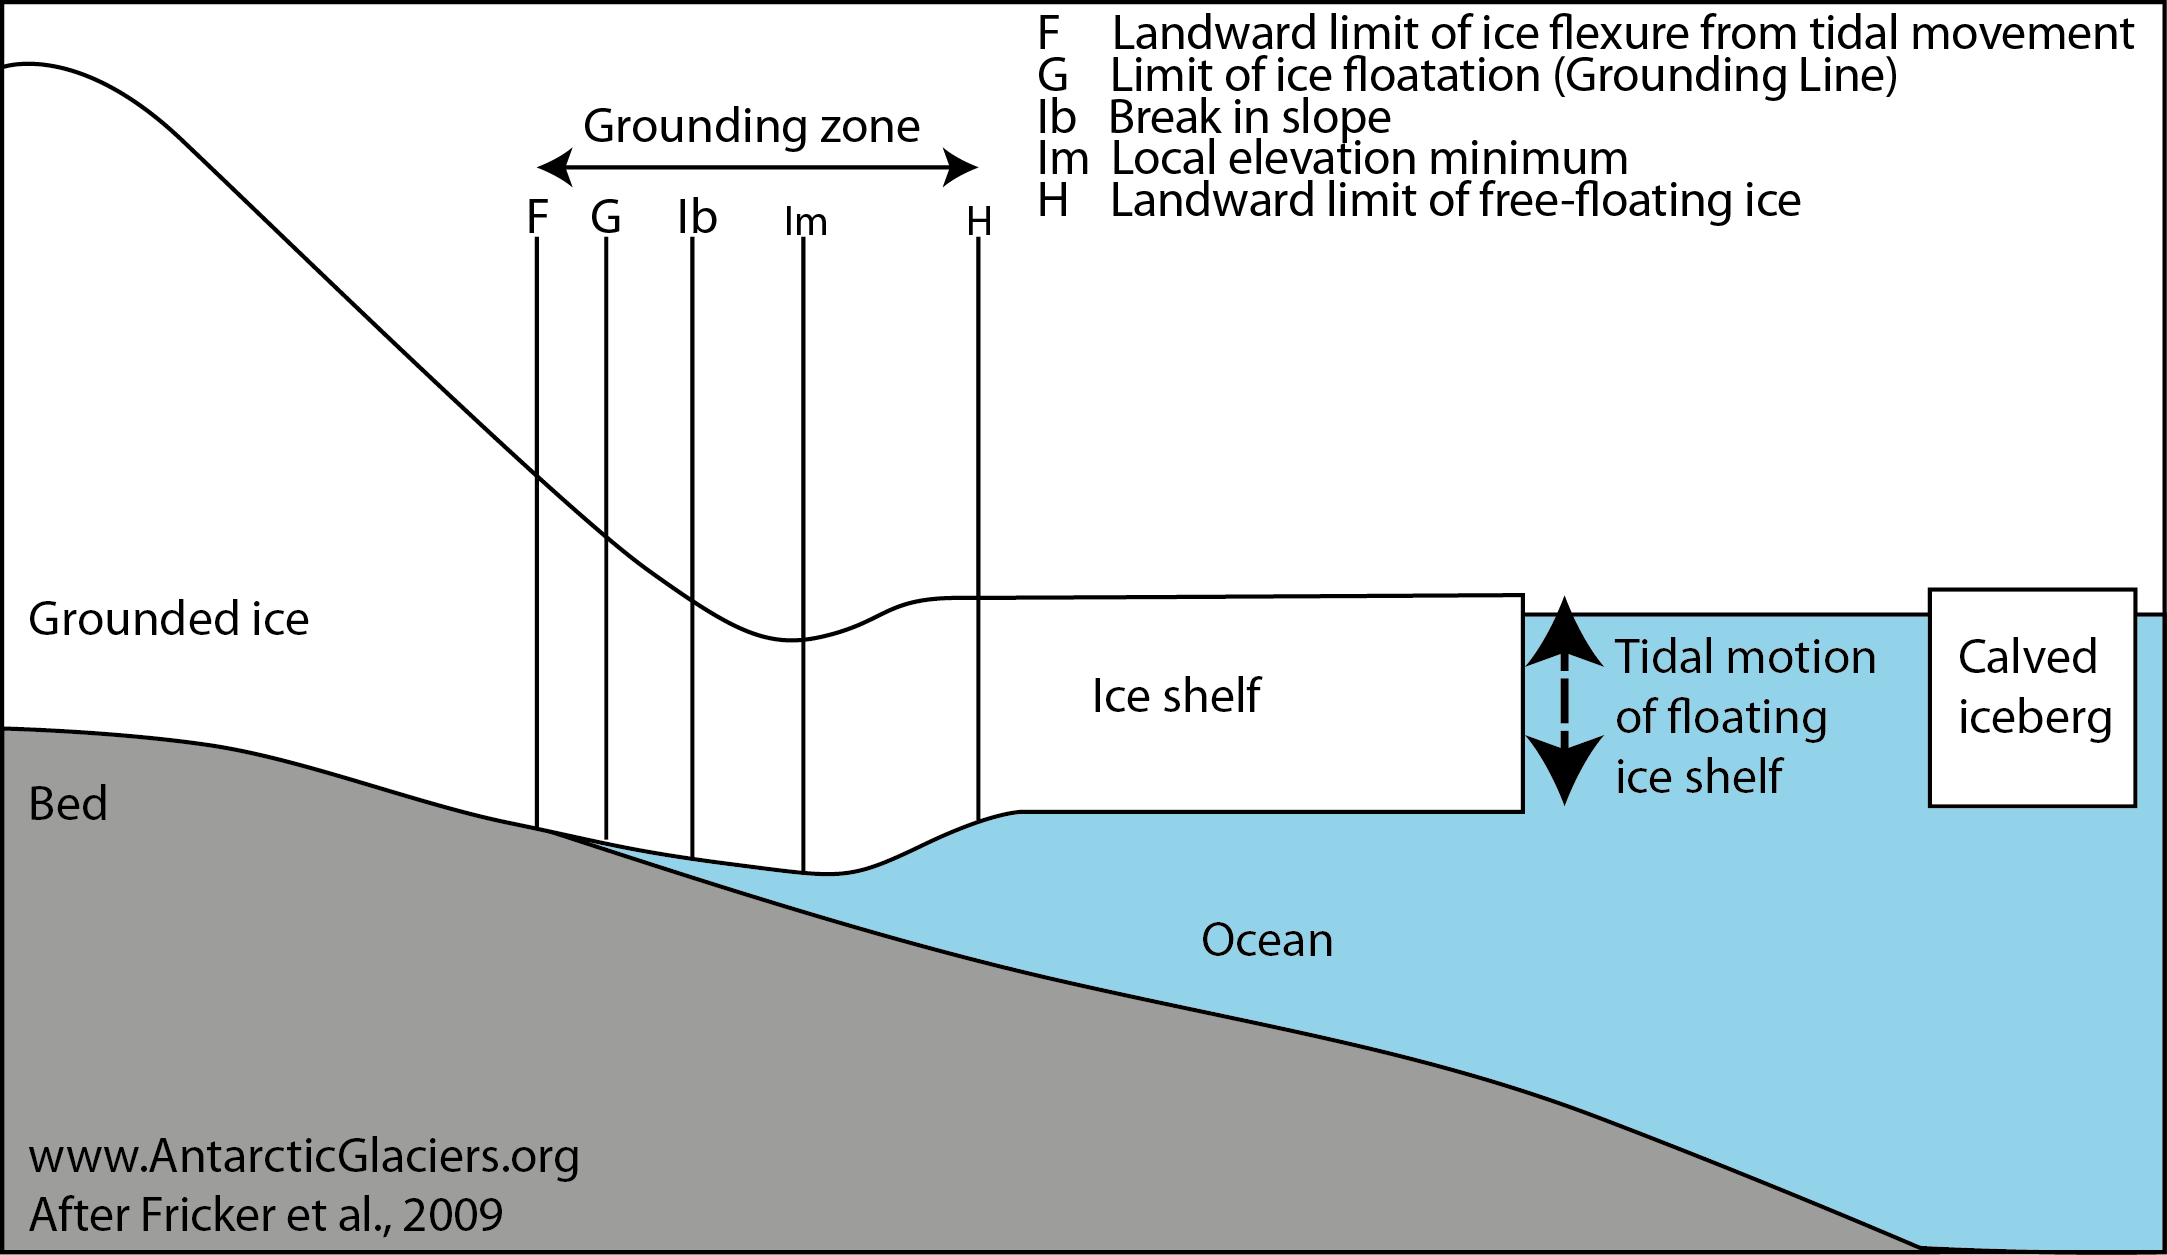
\includegraphics[width=0.7\textwidth]{../fig/groundingzone.png} % \\\includegraphics[width=0.5\textwidth]{topography_x-profile.png}\includegraphics[width=0.5\textwidth]{topography_y-profile.png}
			\caption{\footnotesize Schematic of a tributary glacier where we can observe the different parts denoting the grounding zone (Fricker et al., 2009).}
		\end{figure}
	\end{center}
\end{frame}
\begin{frame}
	\frametitle{Grounding line stability}
		\begin{center}
	\begin{figure}[!h]
		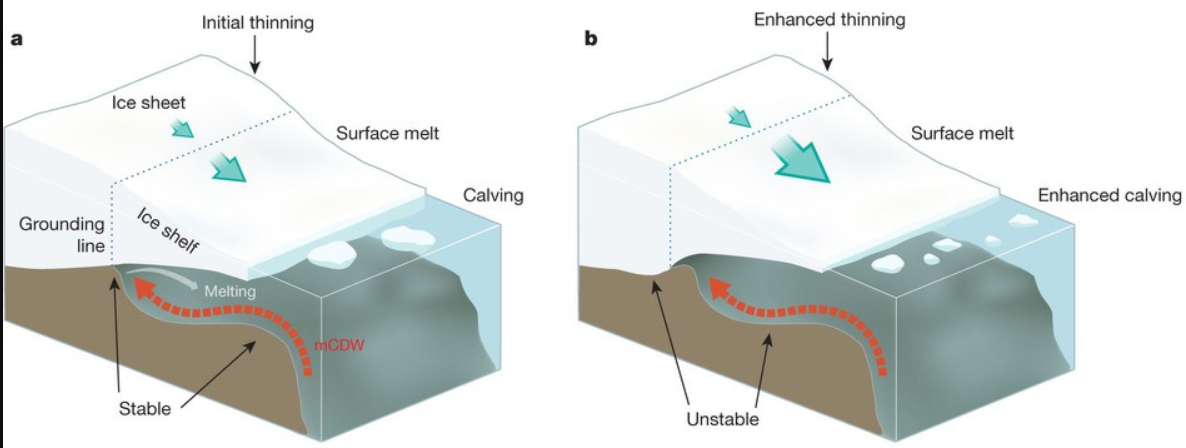
\includegraphics[width=0.7\textwidth]{../fig/MISI.png} % \\\includegraphics[width=0.5\textwidth]{topography_x-profile.png}\includegraphics[width=0.5\textwidth]{topography_y-profile.png}
		\caption{\footnotesize Schematic representation of the marine ice sheet instability with a) an initial state grounding line position and b) an unstable grounding line position (Hanna et al., 2013).}
	\end{figure}
\end{center}
\end{frame}
\begin{frame}
	\frametitle{Objective}
	\begin{itemize}
		\item Understand the direct impact of changes in the position of the grounding line on the flow dynamics of ice sheets glaciers.
		\item We will use the finite element model Elmer/Ice to explore the spatial resolution impact on the grounding line position.
		\item We will compare the changes in the position of the grounding line for two different idealised topographies. This will let us to understand the behavior of real present and past glaciers such as the Northern European glacier. 
	\end{itemize}
\end{frame}

\begin{frame}
	\frametitle{Idealised topographies: cone}
	This numerical experiment uses two different topographic profiles. A cone and a more realistic topography (thule). These idealised topographies are used in the world-wide model intercomparison project CalvinMIP (See \url{https://github.com/JRowanJordan/CalvingMIP/wiki/} for updates).
	\begin{itemize}
	\item Cone: the idealised model consists of a circular bedrock configuration given by:
		\begin{equation}
			\theta=arctan2(y,x);
		\end{equation}
		\begin{equation}
			I=R-cos(2\theta)\frac{R}{2}
		\end{equation}
		\begin{equation}
			Bed_0=Bc-(Bc-BI)\frac{|x^2+y^2|}{R2}^;
		\end{equation}
		Where $R=800x10^3 m$, $Bc=0.9 x 10^3 m$, and $BI=-2 x 10^3 m$. 
	\end{itemize}
\end{frame}
\begin{frame}
	\frametitle{Idealised topographies: cone}
	\begin{center}
			\begin{figure}[!h]
			\centering
			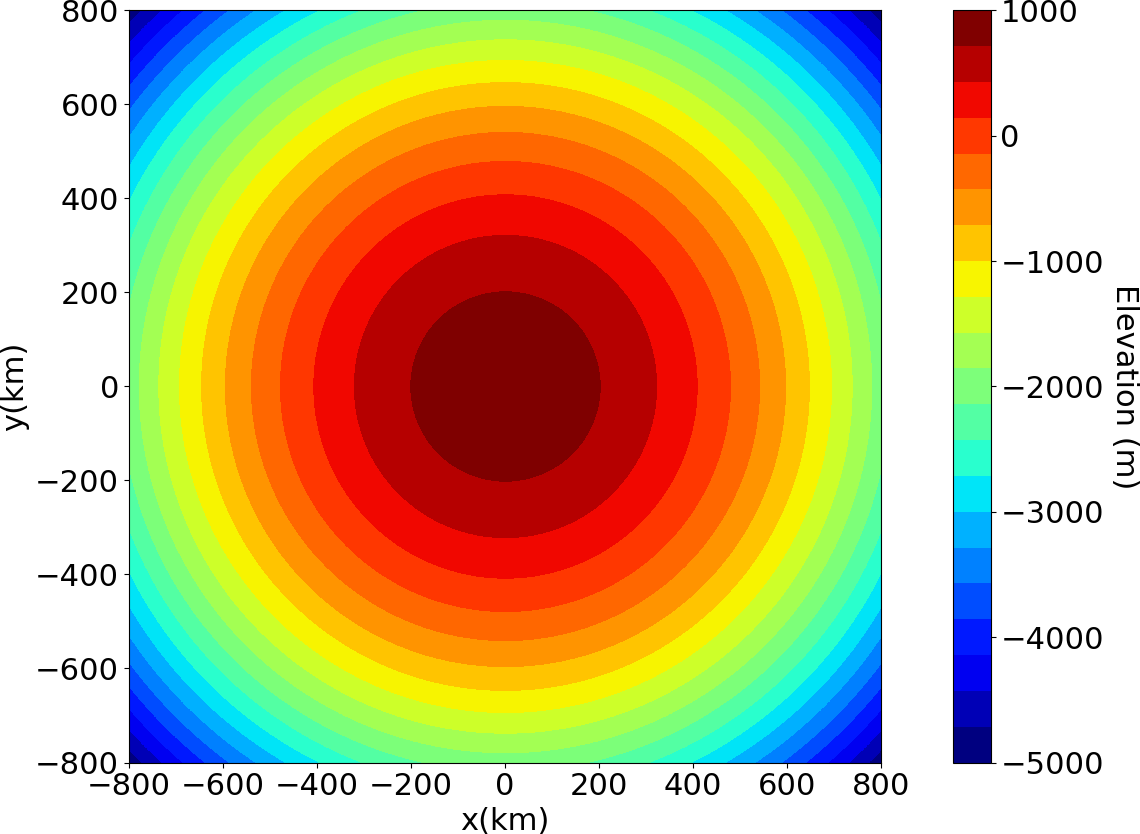
\includegraphics[width=0.45\linewidth]{../fig/circular_topo_top}
			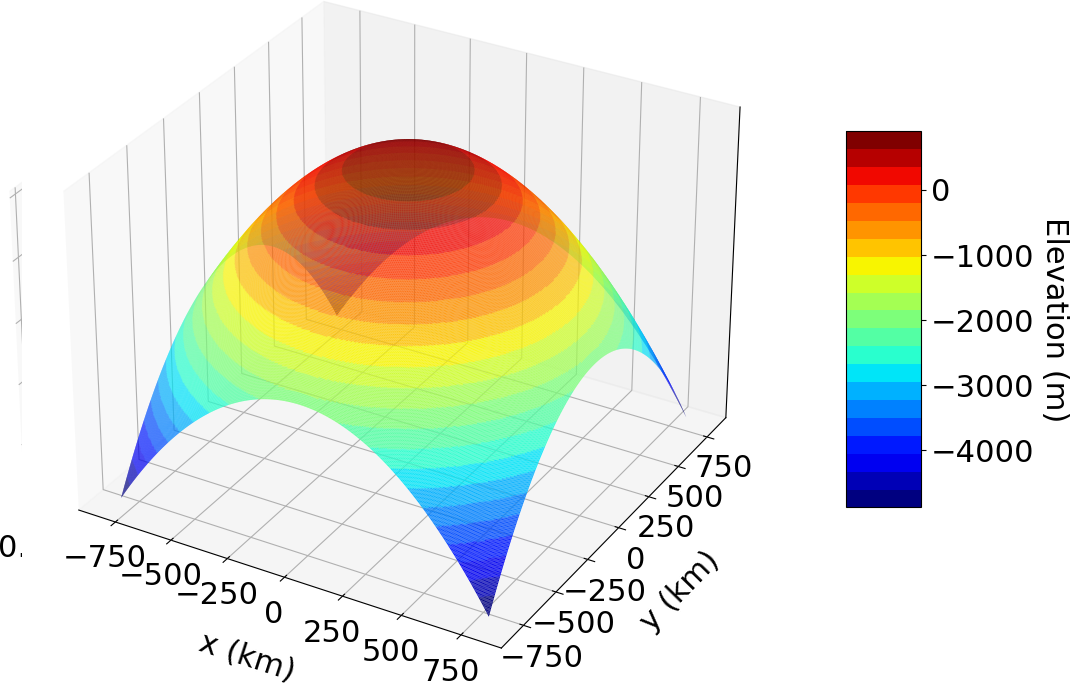
\includegraphics[width=0.45\linewidth]{../fig/circular_topo_jet}
			\caption{Circular bedrock topography. On the left side top view and on the right side, lateral view.}
			\label{circular_topo_top}
		\end{figure}
	\end{center}
\end{frame}
\begin{frame}
	\frametitle{Idealised topographies: thule}
	\begin{itemize}
		\item Thule: The thule bedrock configuration is given by:
			\begin{equation}
			\theta=arctan2(y,x);
		\end{equation}
		\begin{equation}
			I=R-cos(2\theta)\frac{R}{2};
		\end{equation}
		\begin{equation}
			Bed_0=Bc-(Bc-BI)\frac{|x^2+y^2}{R^2};
		\end{equation}
		\begin{equation}
			Bed=Bacos(3\pi\frac{\sqrt[2]{x^2+y^2}}{I})+Bed_0;
		\end{equation}
		With $R=800 x 10^3 m$, $Bc=0,9 x 10^3 m$, $BI=-2 x 10^3 m$, and $Ba=1,1 x 10^3$.
	\end{itemize}
\end{frame}
\begin{frame}
	\frametitle{Idealised topographies}
	\begin{center}
			\begin{figure}[!h]
			\centering
			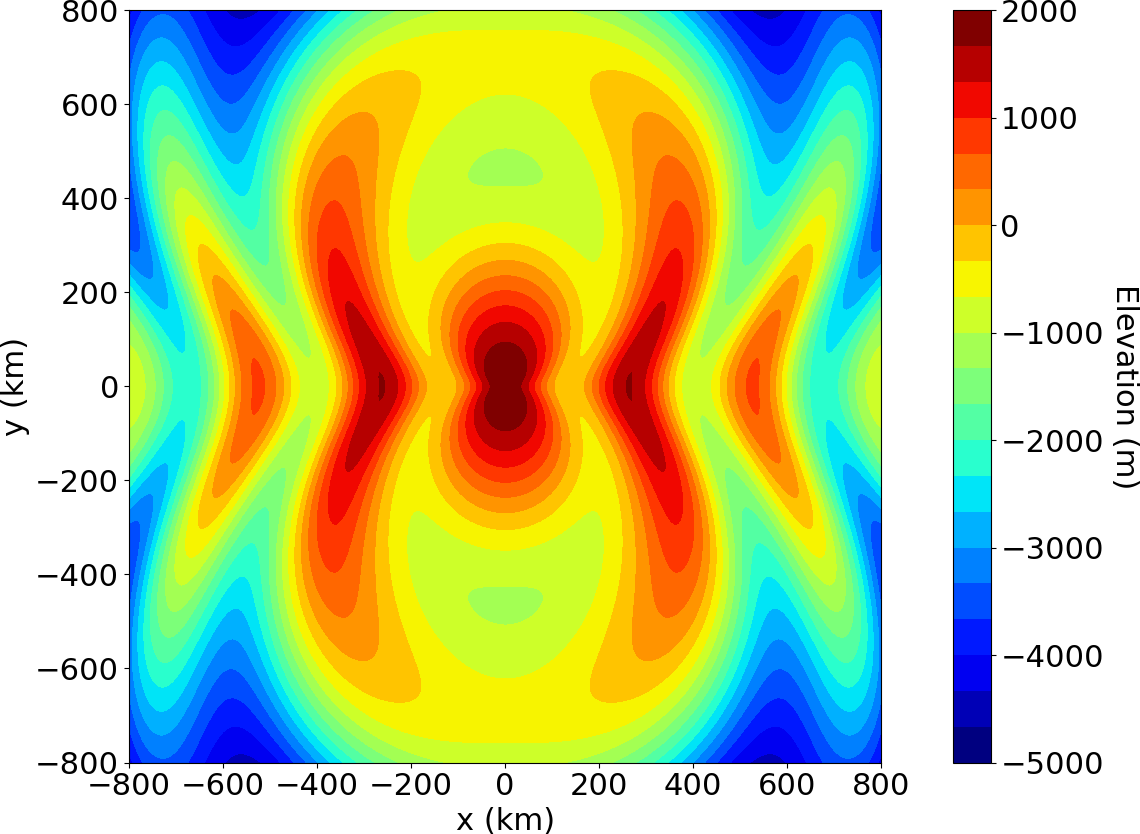
\includegraphics[width=0.45\linewidth]{../fig/Thule_2D}
			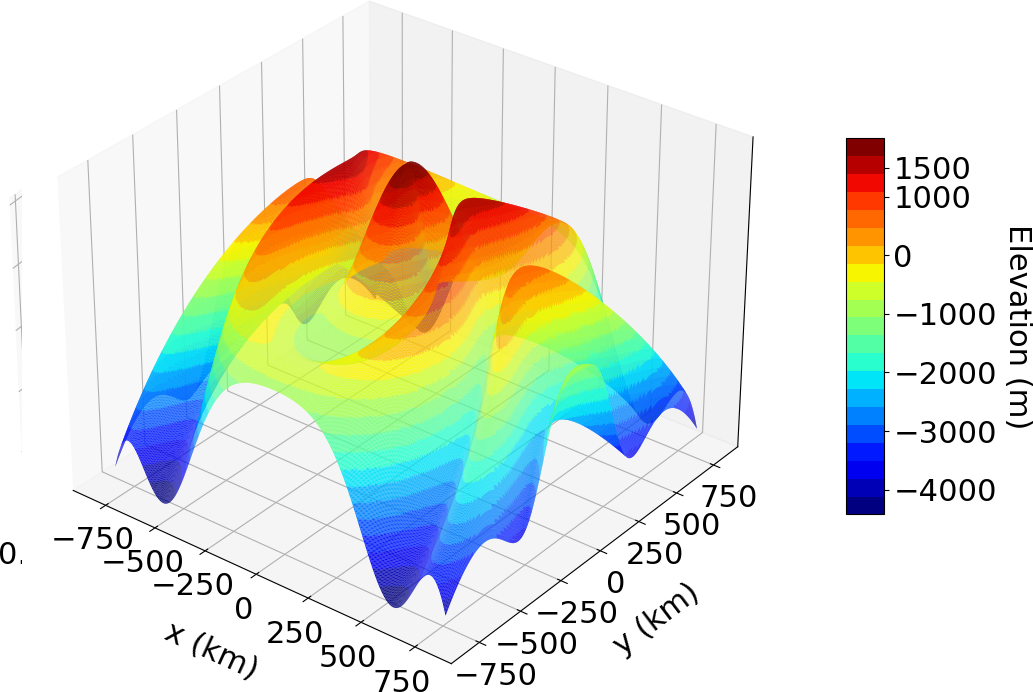
\includegraphics[width=0.45\linewidth]{../fig/Thule_3D}
			\caption{Thule bedrock topography 3D. On the left side the top view, and on the right side a lateral view.}
			\label{Thule_3D}
		\end{figure}
	\end{center}
\end{frame}
\begin{frame}
	\frametitle{Parameters}
	\begin{center}
		\begin{figure}[!h]
			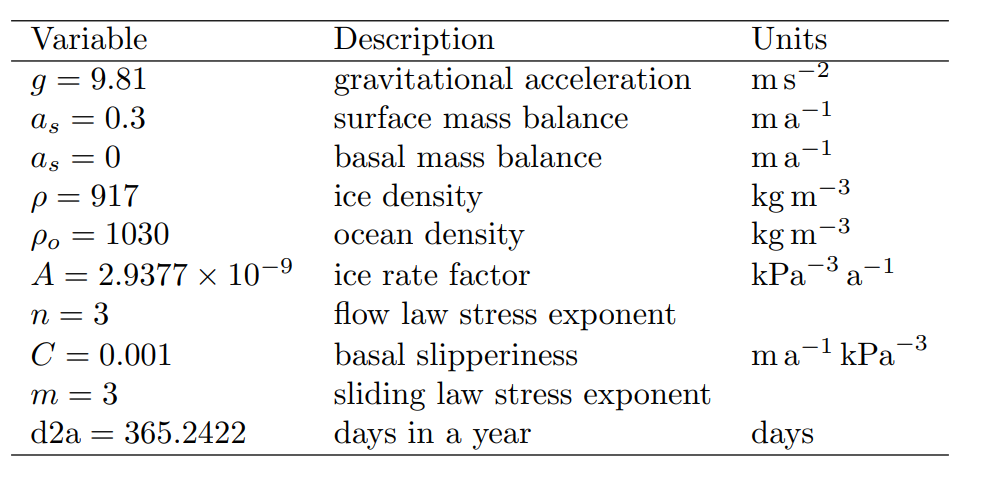
\includegraphics[width=0.7\textwidth]{../fig/Constants_parameters.png} % \\\includegraphics[width=0.5\textwidth]{topography_x-profile.png}\includegraphics[width=0.5\textwidth]{topography_y-profile.png}
			\caption{\footnotesize Constants parameters based on Hilmar Gudmundsson's experiment for thule's configuration, used in MIP experiments. }
		\end{figure}
	\end{center}
\end{frame}
\begin{frame}
	\frametitle{Elmer/Ice finite element method}
\begin{itemize}
	\item 	Open source finite element code, mainly depeloped by the CSC in Finland. 
	\item The ice sheet/ice flow model Elmer/ice is based on Elmer and includes developments related to glaciological problems. Elmer/ice includes a large number of dedicated solvers and users functions.
	\item 	Elmer/ice solves the full-stokes equations for various ice rheologies. 
	It includes solvers for the classical asymptotical expansions of the stokes equations, namely the shallow 	ice approximation (SIA) and the shallow shelf approximation (SSA).
\end{itemize}
\end{frame}
\begin{frame}
	\frametitle{Grid and bedrock}
		\begin{center}
		\begin{figure}[!h]
			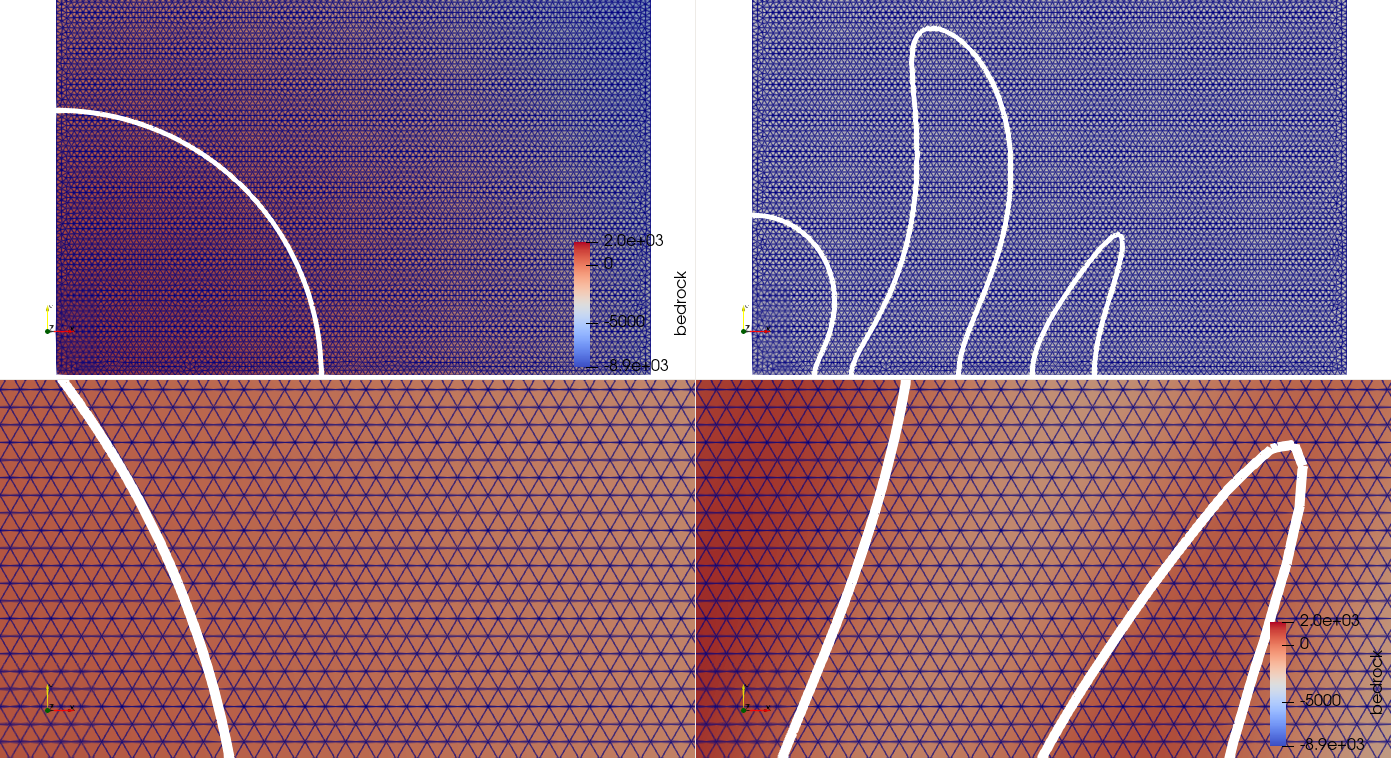
\includegraphics[width=0.7\textwidth]{../fig/grid_and_bedrock.png} % \\\includegraphics[width=0.5\textwidth]{topography_x-profile.png}\includegraphics[width=0.5\textwidth]{topography_y-profile.png}
			\caption{\footnotesize Elmer/Ice grid used to simulate one of the idealised topographies. On the left side the cone topography and on the right side the mesh for the simulation of the thule topography. }
		\end{figure}
	\end{center}
\end{frame}
\begin{frame}
	\frametitle{Boundary conditions}
	\begin{itemize}
		\item The bedrock is impermeable (The vertical component of the ice flow velocity is 0). 
		\item The flow follows Weertman friction law.
		\item Mass acumulation is a constant parameter.
		\item The simulation will be performed on a quarter of the domain, since the geometry of the topography is symmetric, which allows to have free slip boundary condition at the left and down side of the topography, and open boundary condition at the right and top side of the domain. 
	\end{itemize}
\end{frame}
\begin{frame}
	\frametitle{Work plan}
	\begin{figure}[!h]
		\centering
		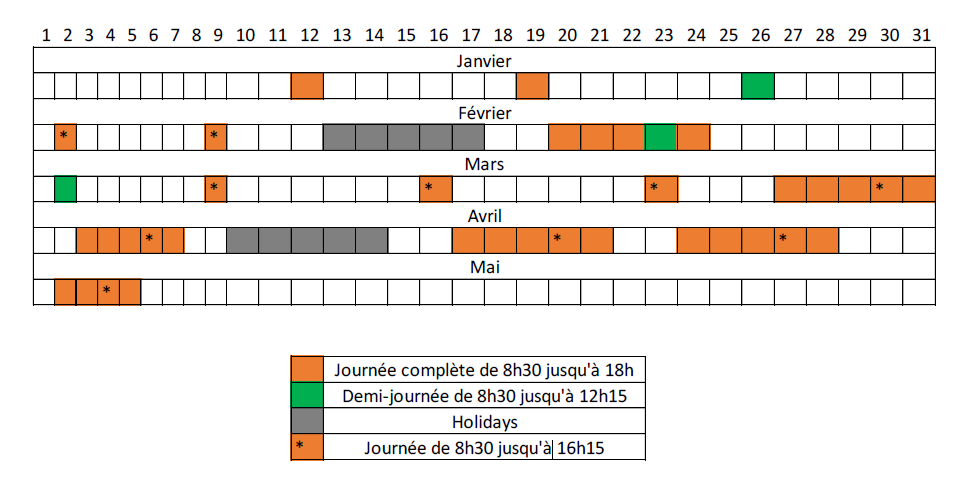
\includegraphics[width=0.7\linewidth]{../fig/Schedule}
		\caption{Tasks schedule of the project, showing the days we will spend working on the different stages of it.}
		\label{Schedule}
	\end{figure}
\end{frame}
\begin{frame}
	\frametitle{Work plan}
January
\begin{itemize}
	\item Second and third week:Running the first idealised simulations.(10km and 5km resolution. 1 and 2 days, respectively.)
\end{itemize}
February
\begin{itemize}
	\item First week: Simulations using a 2km resolution.  (3-4 days.).
	\item Second week: 1km resolution (5 days).
	\item Fourth week: 500m and 250m resolutions (1-2 weeks resp.)
\end{itemize}
March
\begin{itemize}
	\item First, second, and third week: Analysis of the simulations results.
	\item Fourth week: Writing the report.
\end{itemize}
April
\begin{itemize}
	\item  Writing the results.
\end{itemize}
May
\begin{itemize}
	\item Presentation of the results.
\end{itemize}
\end{frame}
\begin{frame}
	\frametitle{Preliminary results}
\begin{center}
	\begin{figure}[!h]
		\centering
		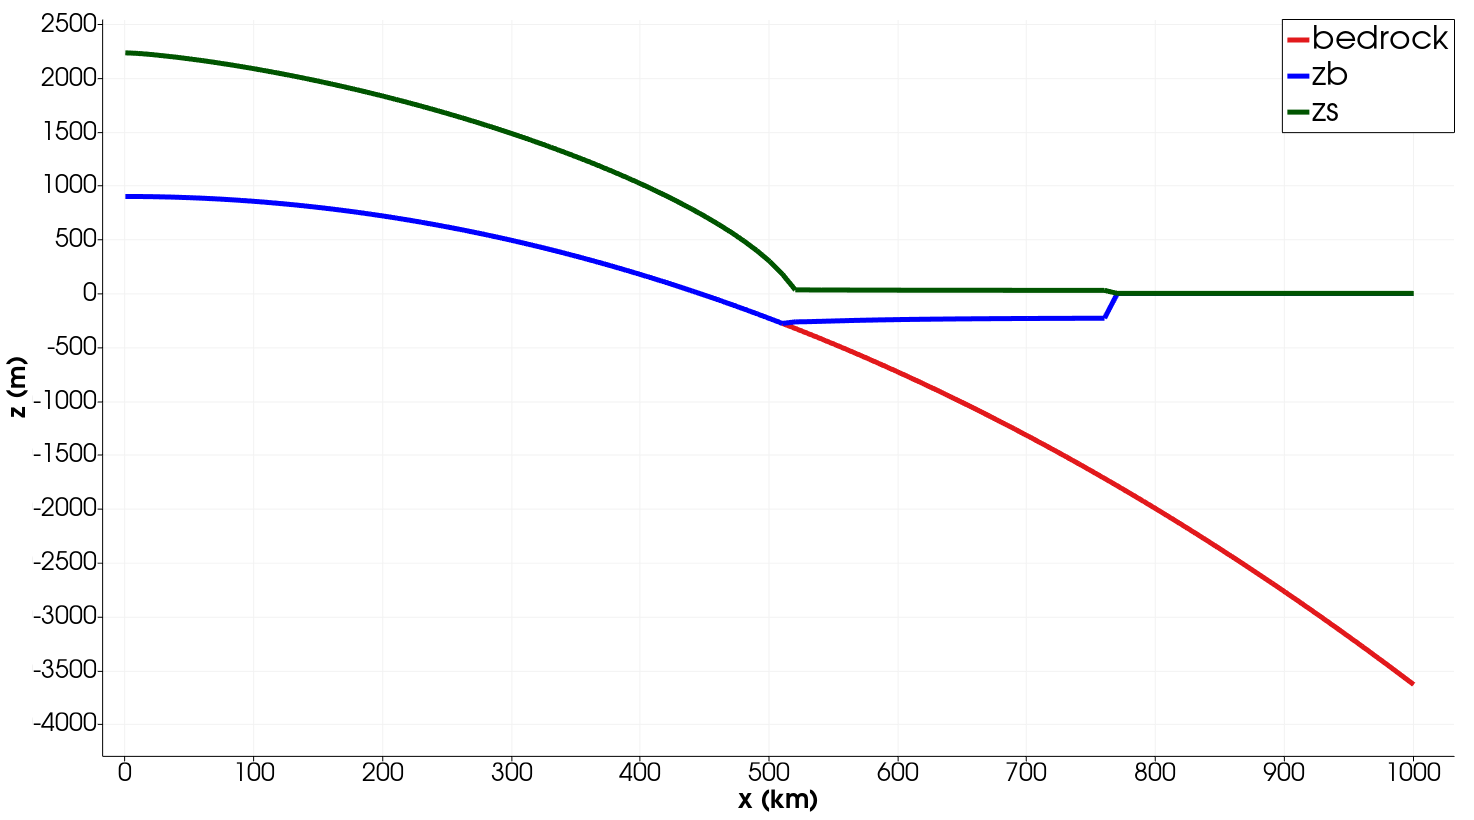
\includegraphics[width=0.45\linewidth]{../fig/cone_grounding_line.png}
		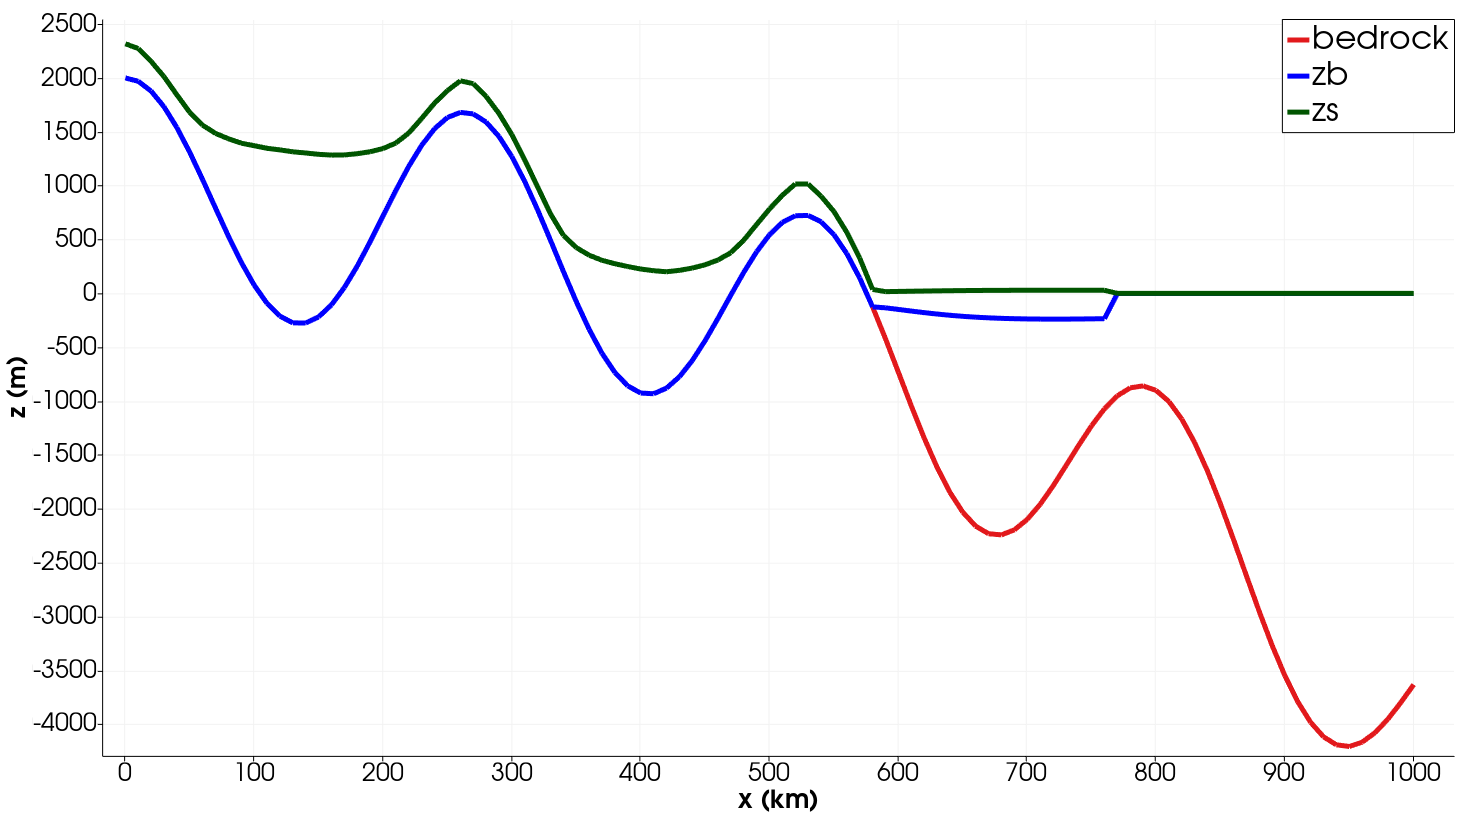
\includegraphics[width=0.45\linewidth]{../fig/thule_grounding_line.png}
		\caption{10 km resolution simulation for cone (left side) and thule (right side) topographies. In green the upper heigh of the ice sheet, in blue the lower heigh, and in red the bedrock position.}
		\label{10kmsimulation}
	\end{figure}
\end{center}
\end{frame}
\end{document}